%!TEX TS-program = XeLaTeX
\documentclass[11pt]{article}

\usepackage{amssymb}
\usepackage{amsthm}
\usepackage{amsmath}
\usepackage{mathtools}

\usepackage{fancyhdr}
\usepackage{graphicx}
\usepackage[top=3cm, left=2cm, right=2cm, headheight = 90pt]{geometry}
\usepackage{xltxtra}
\usepackage[font=small,labelfont=bf]{caption}

%%%%%%%%%%%%%%    Language matters  %%%%

%\usepackage[latvian]{babel}
%\usepackage[L7x]{fontenc}
%\usepackage[utf8x]{inputenc}

%%%%%%%%%%%%%%%%%%%%%%%%%%%%%%%%%%%7%%%%%

%%%%%%%%%%%%%%%%%%%%%%%%%%%       DO NOT EDIT         %%%%%%%%%%%%%%%%%%
%\usepackage{setspace}
%\renewcommand{\headrulewidth}{1pt}
%\fancyhead[L]{\includegraphics[width=3cm]{pictures/logo}}
%\fancyhead[R]{\raisebox{3ex}{\fbox{Language: \bf \lang}}}
\fancyhead[C]{{\Large\bf Recurrences - Problems}\\ \date}

\renewcommand{\theenumi}{\alph{enumi}}
%\newcommand{\problem}[1]{\paragraph{Problem #1.}}%<--------------- TRANSLATE THE WORD "Problem".
\fancyfoot[CE,CO]{}  % this is to remove page numbers (as you might want for single page docs)

\def\leq{\leqslant}
\def\geq{\geqslant}
\def\N{\mathbb N}
\def\R{\mathbb R}
\def\Z{\mathbb Z}
\DeclarePairedDelimiter\ceil{\lceil}{\rceil}
\DeclarePairedDelimiter\floor{\lfloor}{\rfloor}

%%%%%%%%%%%%%%%%%%%%%%%%%%%%%%%%%%%%%%%%%%%%%%%%%%%%%%%%%%%%%%%%%%%%%%%%%


%%% Language name in english %%%%%%%%%
\def\lang{Latvian}

%\def\lang{Lithuanian}

%%%%%%%%%%%%%%%%%%%%%%%%%%%%% TRANSLATE HERE %%%%%%%%%%%%%%%%%%%%%%%%%%%%%%%%%%

%\def\date{2018. gada 18. jūnijs}
%\def\notes{}


%%%%%%%%%%%%%%%%%%%%%%%%%%%%%%%%%%%%%%%%%%%%%%%%%%%%%%%%%%%%%%%%%%%%%%%%%%%%%%%

\def\prob{}

%%%%%%%%%%%%%%%%%%%%%%%%%%%%%%%%%%%%%%%%%%%%%%%%%%%%%%%%

\theoremstyle{definition}
\newtheorem{problem}{\prob}

\pagestyle{fancy}



\begin{document}
%\thispagestyle{fancy}
\noindent 
%\emph{\notes}

%1
\begin{problem}
\textit{[Derangements of hats]}
Suppose there are $n$ people and each has one hat. They all throw hats in a pile and then each takes one hat out of pile. 

How many possible ways are there to do this so that no-one gets his  own hat? 
\end{problem}
%

%2
\begin{problem}
\textit{[Guess - then prove method]}
$
b(0)=0; \quad b(1)=1; \quad
b(n)=b(\floor{\frac{n}{2}})+b(\ceil{\frac{n}{2}})
$
\end{problem}
%

%3
\begin{problem}
\textit{[How to guess - pattern spotting - differences]}
$
a(0)=12; \quad
a(1)=17; \quad
a(n)=a(\floor{\frac{n}{2}})+a(\ceil{\frac{n}{2}})-12
$
\end{problem}
%

%4
\begin{problem}
\textit{[How to guess - pattern spotting - 2nd order differences]}
$
a_0=7; \quad
a_1=12; \quad
a_n=a_{n-2}+8n-2
$
\end{problem}
%

%5
\begin{problem}
\textit{[How to guess - pattern spotting - n-th order differences]}
$
s_0=0; \quad
s_n=s_{n-1}+n^2
$
\end{problem}
%

%6
\begin{problem}
\textit{[How to guess - pattern spotting - ratios]}
$
g_0=2; \quad
g_1=6; \quad
g_n=g_{n-1}+6g_{n-2}
$
\end{problem}
%

%7
\begin{problem}
\textit{[How to guess - pattern spotting - error terms]}
$
a_0=5; \quad
a_n=2a_{n-1}+1
$
\end{problem}
%

%8
\begin{problem}
\textit{[How to guess - pattern spotting in formulas - repeated substitutions]}
$
a_0=5; \quad
a_n=3a_{n-1}+2n
$
\end{problem}

%9
\begin{problem}
\textit{[Linear homogenous recurrences]*}
$
a_0=1; \quad
a_0=1; \quad
a_n=a_{n-1}+a_{n-2}
$
\end{problem}
%

%10
\begin{problem}
\textit{[Linear non-homogenous recurrences]*}
$
a_0=2; \quad
a_0=3; \quad
a_n=a_{n-1}+a_{n-2}+3n+1
$
\end{problem}
%

%11
\begin{problem}
\textit{[Tower of Hanoi]}
\textit{Tower of Hanoi} consists of $3$ rods $A$, $B$ and $C$ and $n$ discs of different sizes. Initially all discs are stacked on one rod so that no disc is placed on top of smaller one.
\begin{center}
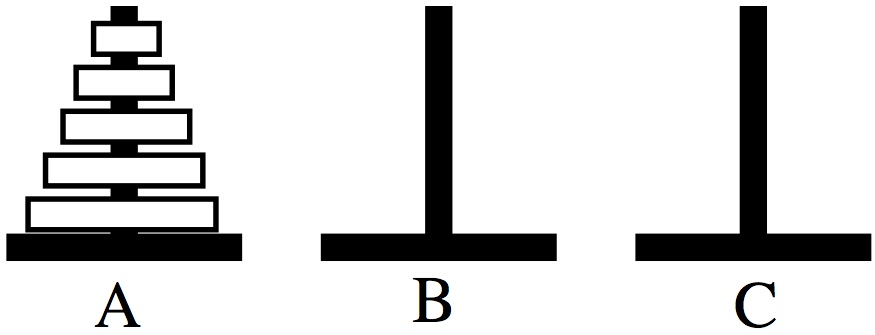
\includegraphics[width=5cm]{TowersOfHanoiFigure.jpg}
\captionof{figure}{Tower of Hanoi }
\label{fig:Hanoi}
\end{center}
The objective is to move the entire stack to another rod, obeying the following simple rules:
\begin{enumerate}
\item Only one disk can be moved at a time.
\item Each move consists of taking the upper disk from one of the stacks and placing it on top of another stack or on an empty rod.
\item No disk may be placed on top of a smaller disk.
\end{enumerate}
What is the minimal number of moves to move all discs from $A$ to $B$?
\end{problem}
%

%12
\begin{problem}
\textit{[Pizza problem]}
How many pieces of pizza is it possible to obtain using $n$ straight cuts?
\end{problem}
%

%13
\begin{problem}
\textit{[Josephus problem]}
$n$ people numbered $1$ to $n$ stand in a circle. Every second person starting from $1$ is eliminated and leaves the circle until only one person remains. 

For a given $n$ what is the number of remaining person?
\end{problem}
%

\end{document}
